\documentclass[12pt]{article}
\usepackage[margin=0.7in]{geometry} 		% defines page margin
\usepackage{knitting} 				% defines \chart and \textknit
\usepackage{titling} 				% title page
\usepackage{graphicx,xspace, scrextend}	% defines space control stuff
\usepackage{tabularx, array, colortbl}	% defines tables
\usepackage{multicol} 				% defines columns
\usepackage{multirow} 				% defines multirows, combined cells in tables
\usepackage{framed} 				% defines boxes for notes and written directions
\usepackage[x11names]{xcolor} 		% extends color library
\pdfmapfile{+knitfont.map}

% font selection
\usepackage{palatino, moresize, sectsty}
\allsectionsfont{\sffamily}

\renewcommand{\arraystretch}{2} % compresses tables for pattern keys

\newcolumntype{L}[1]{>{\leftalign\arraybackslash}p{#1}}
\newcolumntype{C}[1]{>{\centering\arraybackslash}p{#1}}

% length parameters
\setlength{\parindent}{0pt} % disables indentation for paragraphs
\setlength{\columnsep}{0.7cm} % column separation in multicol environment

% color parameters
\colorlet{framecolor}{black}
\colorlet{shadecolor}{LemonChiffon1}
\colorlet{highlight}{yellow}

% COLORWORK?!
\colorlet{MC}{purple!50}
\colorlet{CCA}{green}
\colorlet{CCB}{white}

\newcommand{\makeActive}{
	\catcode`\0=\active % MC
	\catcode`\1=\active % CC1
	\catcode`\2=\active % CC2
}	% define additional colors as needed

% plain knit colorwork symbols are defined with charts
% how to get other symbols (increases/decreases)
\newcommand{\MC}[1]{\purlpass{\color{MC}}\purlbackground{#1}}
\newcommand{\CCA}[1]{\mainpass{\color{black}}\purlpass{\color{CCA}}\purlbackground{#1}}
\newcommand{\CCB}[1]{\mainpass{\color{black}}\purlpass{\color{CCB}}\purlbackground{#1}}

% custom commands
\newcommand{\comment}[1]{} % allows for multiline comments that LaTeX will ignore

\newcommand{\vocab}[1]{\emph{\textbf{#1}}} % format for highlighting definitions of stitches, vocabulary terms
\newcommand{\rowDir}[1]{\textbf{#1:}} % indent for written instructions within paragraphs

\renewcommand{\repeat}[1]{\textbf{[#1]}} % format for written repeats, bold with *[ stitches ]*
\newcommand{\x}{$\times$}			% times symbol but shorthand
\newcommand{\setrepeat}[2]{\repeat{#1} #2 times}		% format for repeats with set number of repetitions, bold with [ stitches ]

\newcommand{\blank}{\underline{\hspace{2em}} } % written instructions, fill-in-the-blank box
\newcommand{\highlighted}[1]{\colorbox{highlight}{#1}} % written instructions, highlight particular text


% stitch count commands
\newcommand{\increase}[1]{(\emph{+#1 
	\ifnum#1=1{st}\else{sts}\fi})}
\newcommand{\decrease}[1]{(\emph{$-$#1
	\ifnum#1=1{st}\else{sts}\fi})}
\newcommand{\stitchcount}[1]{(\emph{#1 sts})}

% marker instructions
\renewcommand{\pm}[1]{\emph{pm #1}} % place stitch marker
\newcommand{\sm}{\emph{sm}} % slip marker
\renewcommand{\rm}[1]{\emph{rm #1}} % remove stitch marker

% thick horizontal line
\makeatletter \newcommand{\thickhline}{
    \noalign {\ifnum 0=`}\fi \hrule height 1.5pt
    \futurelet \reserved@a \@xhline
}
\makeatother

% custom environments
\newenvironment{frnote}
    {% framed environment for pattern notes
    	\setlength{\FrameRule}{1.5pt}
    	\def\FrameCommand{\fboxrule=\FrameRule\fboxsep=\FrameSep \fcolorbox{framecolor}{shadecolor}}
    	\MakeFramed {\FrameRestore}}
    {\setlength{\FrameRule}{1pt}
	\endMakeFramed}

\newenvironment{frdirection}
    {% framed environment for written directions
	\def\FrameCommand{\fboxrule=\FrameRule\fboxsep=\FrameSep \fbox}
   	\MakeFramed {\advance\hsize-\width \FrameRestore}
    	\addmargin[1.5cm]{0pt}}
    {\endaddmargin
	\endMakeFramed}

\newenvironment{unframed}
    {% unframed environment for written directions
	\begin{addmargin}[2em]{0pt}
	\setlength{\parindent}{-2em}}
    {%\vspace{1em}
	\setlength{\parindent}{0em}
	\end{addmargin}}

\title{Druid Crown} % pattern name here
\author{Shanel Wu (Piper Nell)}

\begin{document}

%%%%%%%%%%%%%%%%%%%%%%%%%%%%%%%%%%%%%%%%%%%%%%%%%%
% TITLE PAGE 
\small

% COVER PHOTO
% uncommend line below if you want a background fill image
% \ThisLRCornerWallPaper{1.0}{image.jpg} 

{\fontfamily{qag}\selectfont
\HUGE\textbf{\thetitle}
\normalsize(slouchy)
\hspace{\fill} % adjust this space
\theauthor
}

\raggedright
\begin{multicols}{2}
% PICTURE
\includegraphics[width=0.9\linewidth]{worn2}

% Cute description here
~\\
The leaf-inspired colorwork on this hat evokes the druid's primal magics, drawn from the land. This companion hat to the Druid Circle sweater lets you practice your stranded colorwork! Already knit the sweater? You can use your leftover yarn!

\subsection*{Sizing}

Fits preemie (0mo, 6mo, 12mo) \textbf{(child/adult S, adult M, adult L)} heads with options for either a close-fitting beanie or slouchy hat. 
Sizes correspond to head circumferences of 12 (14, 16, 18) \textbf{(20, 22, 24)} in or 30 (35, 40, 45) \textbf{(50, 55, 60)} cm.
Larger sizes can be obtained by following the modification instructions.

% sample measurements, gauge, notes on ease, etc.
\subsection*{Gauge}

6 sts x 8 rows = 1"/2.5cm or 24 sts x 32 rows = 4"/10cm in stockinette with size A needles and MC, after gentle blocking.

\subsection*{Yarn Requirements}

% yardage, number of colors, etc.

% also include: sample yarn, other yarn suggestions
Sport or DK weight yarn in a main color (MC) and two contrasting colors (CC1 and CC2)

\textbf{MC:} 60 (70, 100, 130) \textbf{(170, 200, 250)} yds

\textbf{CC1:} 15 (20, 25, 25) \textbf{(30, 30, 35)} yds

\textbf{CC2:} 20 (25, 30, 30) \textbf{(35, 35, 40)} yds

\vfill
\columnbreak
\subsection*{Tools}

\begin{itemize} % NEEDLES
\item 16" circular needle in \textbf{Size A} needed to obtain gauge, for main fabric. \emph{Suggested: US 4/3.5mm} 
\item DPN's in \textbf{Size A} for crown decreases.
\item 16" circular needle in \textbf{Size B} one size smaller than A, for ribbing.
\item tapestry needle
\item stitch markers % MARKERS
\end{itemize}

\subsection*{Techniques}

This pattern is suitable for an advanced beginner with some familiarity with stranded colorwork.
Prior to knitting this pattern, you should be comfortable with knitting in the round, increasing \& decreasing, and simple stranded colorwork. Colorwork is charted only, with no floats longer than 5 stitches. 

~\\
Some support is provided for modifying hat for slouchiness.
Pattern Key describes all abbreviations and describes stitches used.

~\\
\vfill \raggedleft
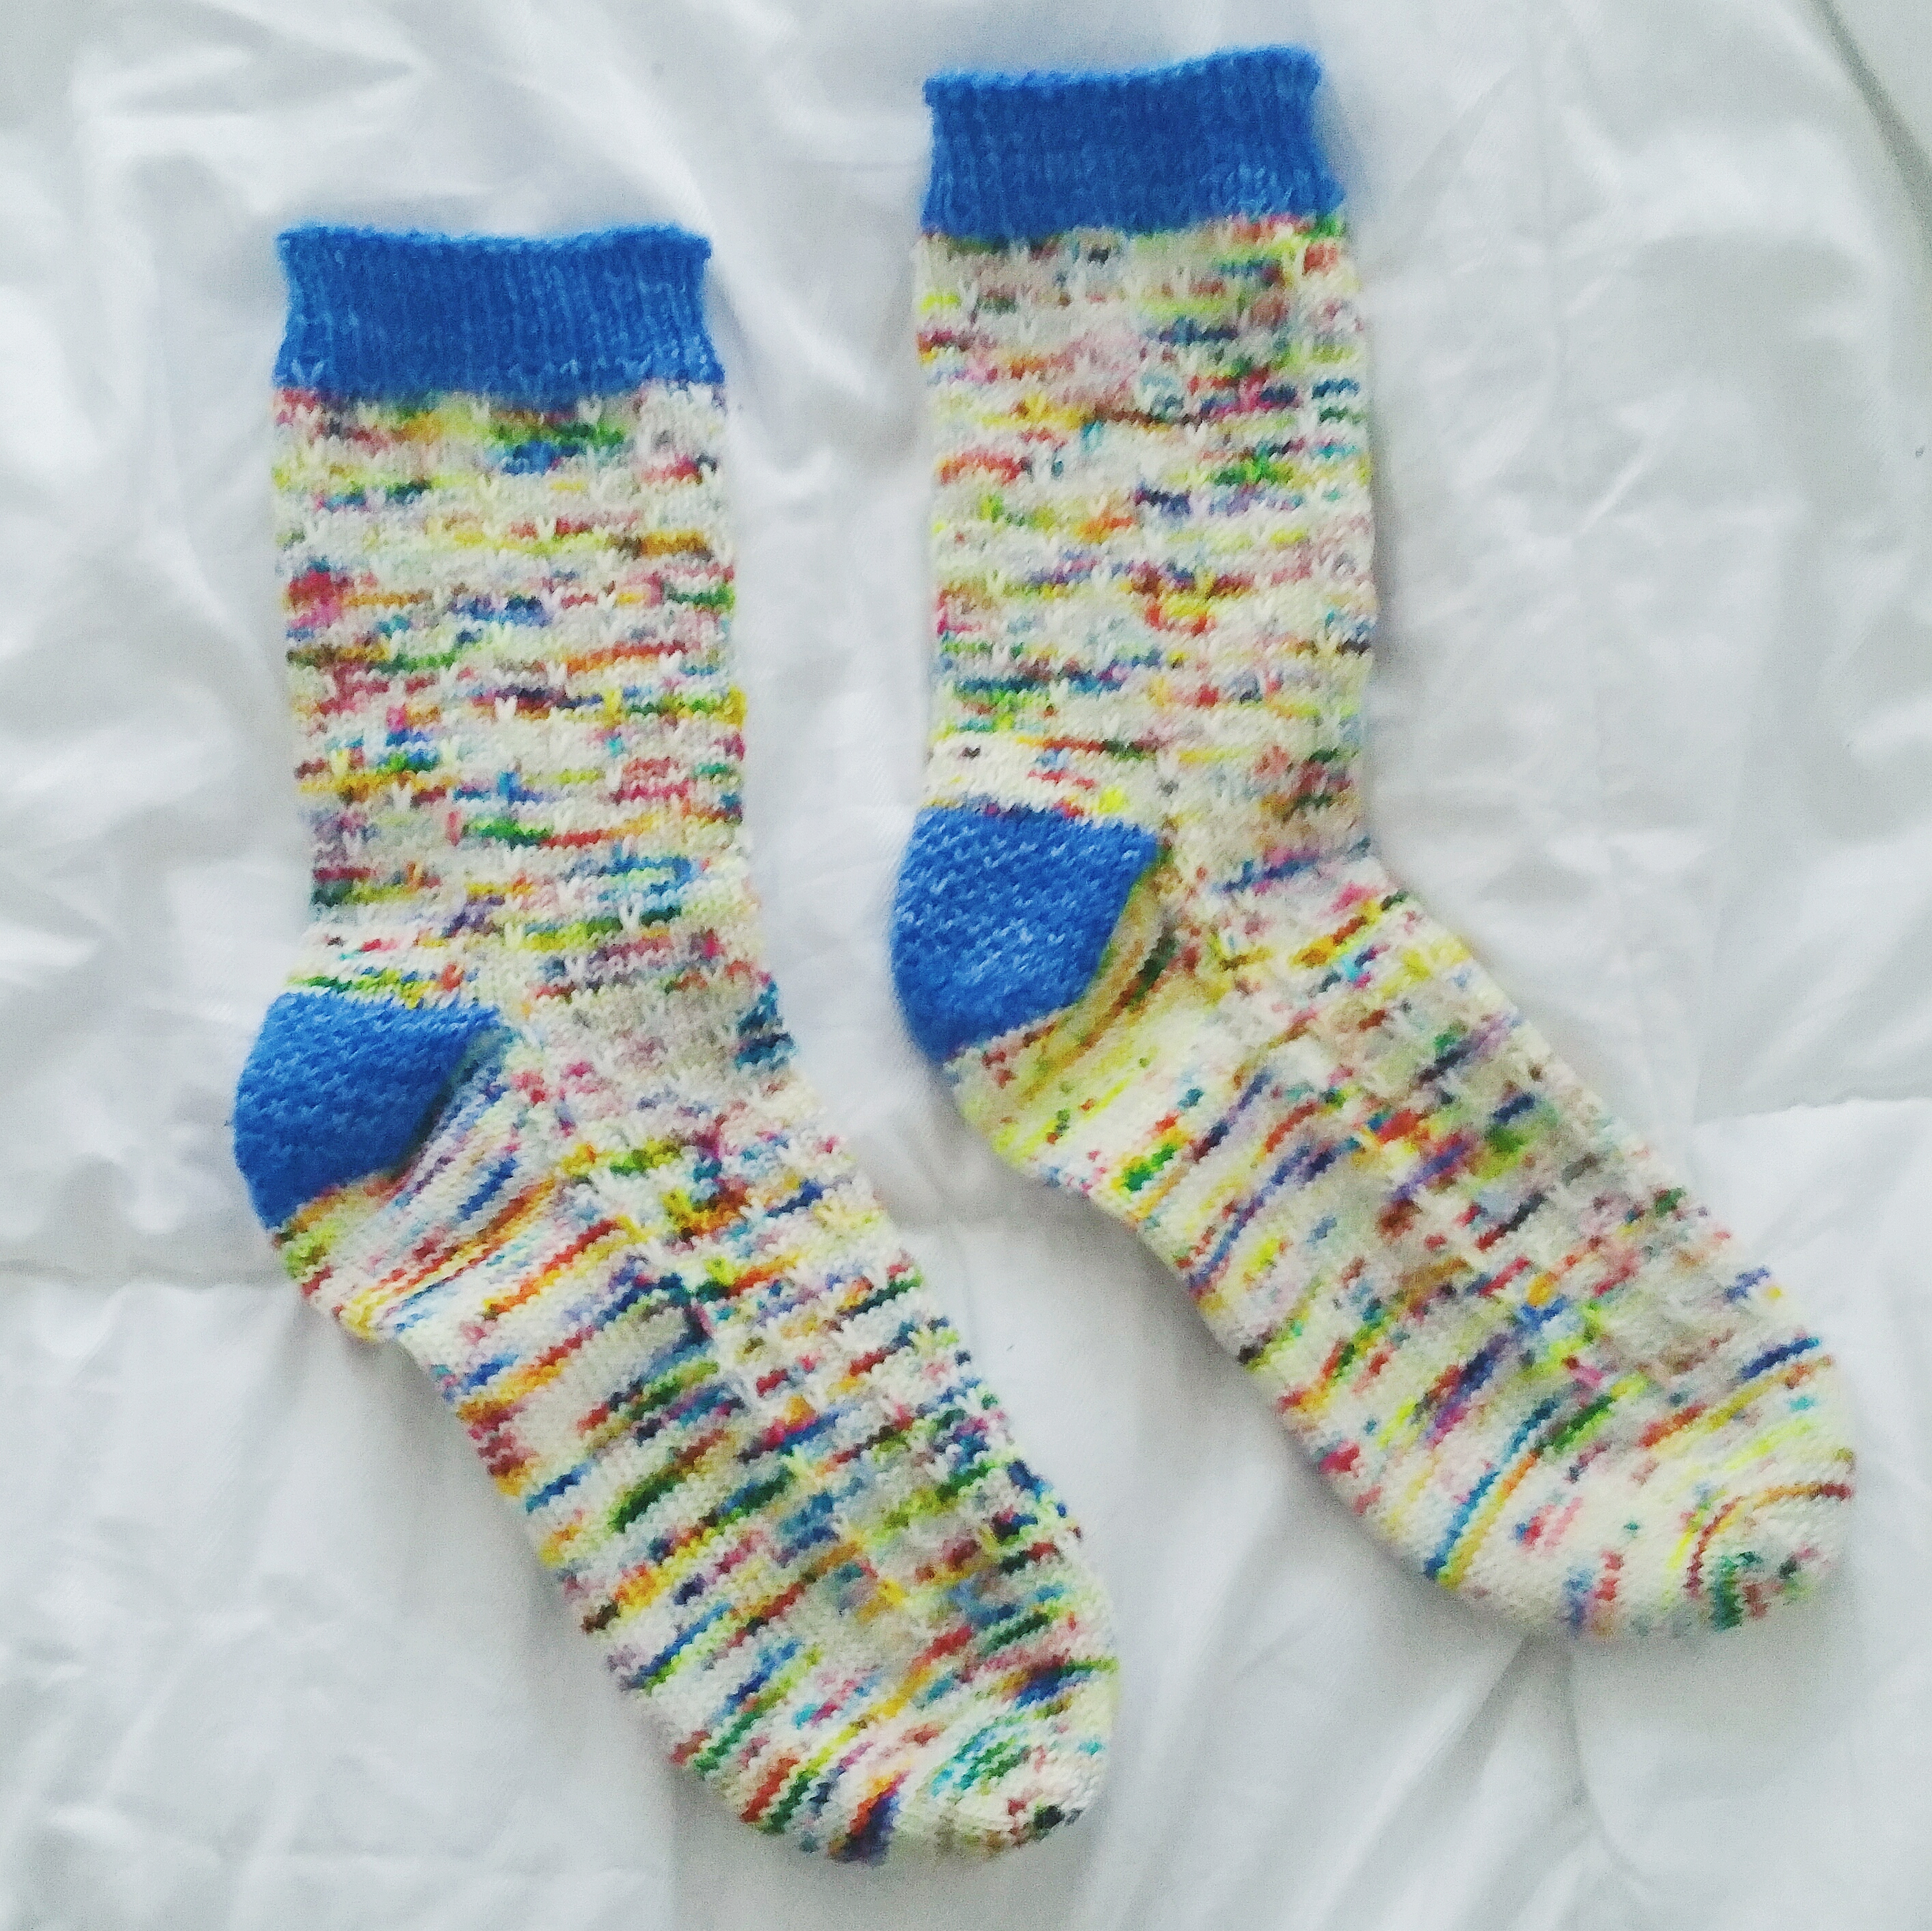
\includegraphics[width=0.7\linewidth]{laidFlat.jpg}

\begin{addmargin}[0.3\linewidth]{0em}
\raggedleft\emph{\ssmall Sample uses BMFA Woobu for MC and North Light Fibers Water Streek DK for CC1 and CC2. Sample shows an Adult M beanie, with extra rounds worked before and after the colorwork to add height, using the 10-point spiral decreases.}
\end{addmargin}
\newpage \raggedright
\subsection*{Pattern Key}

% formatting notes for charts and written directions
\vocab{Written instructions:} repeats = \repeat{stitches}

% abbreviation key - fill in with all abbreviations/stitch patterns used in design: written abbreviation, full stitch name or explanation
% try to keep them in sequential order as they appear in the pattern, or in an order that builds upon previous definitions
% chart symbols included in separate keys attached to their respective charts
% stitches with explanations must first be BOLDED, followed by colon then explanation
\begin{center}
{\renewcommand{\arraystretch}{1.1}
\begin{tabular}{| C{0.2\linewidth}  p{0.6\linewidth} | }
\thickhline \rowcolor{shadecolor} 
\textbf{Written}	& \textbf{Description} \\ \thickhline
CO	& cast on \\
BO 	& bind off \\
BOR 	& beginning of round \\
MC 	& main color \\
CC1 	& contrast color 1 \\
CC2 	& contrast color 2 \\
pm	& place stitch marker \\
sm	& slip stitch marker \\
rm 	& remove stitch marker \\
k	& knit \\
p	& purl   \\
k tbl	& knit through the back loop \\
k2tog 	& knit 2 together \\
m1	& \textbf{make one:} with L needle, pick up bar between sts front to back, k tbl \\
st st 	& \textbf{stockinette stitch:} (worked in the round) k all sts \\
1x1 twisted ribbing 	& \repeat{k tbl, p1} to end of round \\
\hline
\end{tabular}
}
\end{center}
\normalsize

%%%%%%%%%%%%%%%%%%%%%%%%%%%%%%%%%%%%%%%%%%%%%%%%%%
% BEGIN INSTRUCTIONS
\section*{Cast On and Ribbing}

With Size B needles and MC, CO 60 (70, 80, 90) \textbf{(110, 120, 130)} sts with a stretchy cast on. Pm for BOR and join in the round. Work 1x1 twisted ribbing for 0.5 (1, 1, 1) \textbf{(1, 1.5, 1.5)}" or 2.5 (2.5, 2.5, 2.5) \textbf{(2.5, 3.75, 3.75)} cm.

\section*{Main Body}

Change to Size A needles and k one round. 

\vspace{-1em}
\subsection*{Increases \emph{(slouchy only)}}

Work Increase Round once, then k one round.

\textbf{Increase Round:} \repeat{K 6 (7, 8, 9) (11, 12, 13) sts, m1} to end of round. \increase{10}

\begin{frnote}
\vocab{Adult S, M, and L only:} Work Increase Round once more, k one round.
\end{frnote}

Upon completing the slouchy increases, you should have 70 (80, 90, 100) \textbf{(130, 140, 150)} sts total. Proceed to colorwork.

\subsection*{Colorwork}

Join CC1 and CC2. Work chart rows 5-25 (5-25, 1-25, 1-25) \textbf{(1-31, 1-31, 1-31)} repeating a total of 7 (8, 9, 10) \textbf{(13, 14, 15)} times around.

~\\
% CHART
\footnotesize
\begin{tabular}{rl}
\includegraphics[height=370pt]{brackets.png} \hspace{-2em} &
% CHART
{\makeActive
\gdef0{\leavevmode{\purlpass{\color{MC}}=}}
\gdef1{\leavevmode{\purlpass{\color{CCA}}=}}
\gdef2{\leavevmode{\purlpass{\color{CCB}}=}}
\chart[right]{
\mainpass{\color{black}}
\gridpass{\color{gridcolor}}
0020000200
0000000000
2000220002
0111001110
0202002020
0000000000
0001000110
0010011100
0100111100
1001111000
0001110001
0011100010
2211222122
2212221222
1122212211
2212122122
1221221221
2212122122
1122212211
2212221222
2211222122
0011100010
0001110001
1001111000
0100111100
0010011100
0001000110
0000000000
0022000220
0111101111
0200202002
}} \\
\end{tabular}
\normalsize

~\\
After the last row of the chart, work st st until the piece measures 4.5 (4.75, 5.25, 6) \textbf{(6.25, 7, 7.75)}" or 11.5 (12, 13, 14.5) \textbf{(15.5, 17.5, 20)} cm from CO.

\vfill ~\\
\newpage
\section*{Crown Decreases}

\subsection*{Option A: 10-Point Spiral}

\rowDir{Set Up Round} sm, \repeat{k 7 (8, 9, 10) (13, 14, 15) sts, pm} 9 times, k to end of round. This divides the round into 10 equal sections.

\rowDir{Round 1} \repeat{sm, k to 2 sts from marker, k2tog} to end of round. \decrease{10}

\rowDir{Round 2} k all sts.

Work Rounds 1 and 2 a total of 5 (6, 7, 8) \textbf{(11, 12, 13)} times. You will have 20 sts left, or 2 stitches per section.

\rowDir{Next Rnd} sm, \repeat{k2tog, rm} to end of round.

\subsection*{Option B: 5-Point Star}

\rowDir{Set Up Round} sm, \repeat{k 14 (16, 18, 20) (26, 28, 30) sts, pm} 4 times, k to end of round. This divides the round into 5 equal sections.

\rowDir{Round 1} \repeat{sm, k2tog, k to 2 sts from marker, ssk} to end of round. \decrease{10}

\rowDir{Round 2} k all sts.

Work Rounds 1 and 2 a total of 5 (6, 7, 8) \textbf{(11, 12, 13)} times. You will have 20 sts left, or 4 sts per section.

\rowDir{Next Rnd} sm, \repeat{k2tog, ssk, rm} to end of round. 

\section*{Last Round and Finishing}

Both methods of crown decreases end with 10 sts total. Remove BOR marker, then work k2tog 5 more times to end with 5 sts. 

Break yarn, leaving a 6-8" or 15-20cm tail. Using a tapestry needle, thread yarn through all remaining sts and pull tight to close off hat. Weave in all ends and lightly block if desired.

\vfill
\begin{frnote}
\ssmall Pattern \copyright 2019 Shanel Wu. All rights reserved. In purchasing this pattern, you agree to print and use this pattern only for personal use. Do not redistribute or sell paper or electronic copies of this pattern.
\end{frnote}
\columnbreak
%%%%%%%%%%%%%%%%%%%%%%%%%%%%%%%%%%%%%%%%%%%%%%%%%%
% APPENDICES (IF ANY)
\section*{Modification Suggestions}

\subsection*{Custom Sizing Guide}

\emph{\small This guide assumes that you are using the gauge specified by the pattern. For suggestions on how to use a different gauge, see the next section.}

Measure the \textbf{head circumference} at the widest point: \hfill [\#1] \underline{\hspace{5em}}

Subtract 1-2" / 2.5-5cm from \#1 depending on desired amount of negative ease in the brim. Multiply this measurement by the stitch gauge, 6 sts (divide by 2.5 if you are using cm). Round to the nearest \emph{multiple of 10} to obtain the \textbf{CO st count}: \hspace{\fill}[\#2] \underline{\hspace{4em} sts}

Measure the desired \textbf{height}, from the base of the ear to the center of the crown:\hspace{\fill} [\#3] \underline{\hspace{3em}}

Divide \#1 by $6.28$ or $2\pi$ to obtain the \textbf{radius}:\\ \hfill [\#4] \underline{\hspace{5em}}

Then, subtract \#4 from \#3 to obtain the \textbf{pre-decrease height} (i.e. when to begin crown decreases): \hfill [\#5] \underline{\hspace{5em}}

~\\
CO in MC and work ribbing to desired length. If desired, work plain st st to add height or increase evenly by 10's for slouch. Work colorwork chart, then work st st until work is at the height calculated for \#5. Choose a crown decrease method and divide stitches into either 5 or 10 equal sections with stitch markers. Work crown decreases as written.

\subsection*{Substituting Gauge}

If you are looking to knit the pattern at a different gauge, you can follow the custom sizing guide mostly as it's written, changing the calculations for \#2 and \#4. Carefully measure both your stitch gauge and row gauge. If the ratio of stitches to rows is not 3:4, the colorwork and decreases may be distorted.

~\\
When calculating the CO st count (\#2), multiply by your stitch gauge instead of 6. Calculate \#4 by dividing your final stitch count by 5, then by your row gauge. Subtract this length from \#3 to obtain \#5.\end{multicols}
\end{document}